\chapter{Itô and Stratonovich Calculus}

Having established the framework of Itô equations, we now turn our attention to the fundamental problem of change of variables in stochastic calculus. When dealing with deterministic differential equations, the chain rule provides a straightforward mechanism for transforming variables. However, in the stochastic setting, the irregular nature of Brownian motion necessitates a more sophisticated approach.

\section{Itô's Lemma: The Stochastic Chain Rule}

Consider an SDE in Itô form:
$$
dx = a(x)dt + b(x)dW
$$
Suppose we wish to perform a transformation from $x$ to $y$ defined by $y = \psi(x)$. Our objective is to derive an equation of similar form for the transformed variable $y$.

Following the classical approach, we expand $dy$ in a Taylor series:
$$
\begin{array}{rl}
dy & = \psi'(x)dx + \frac{1}{2}\psi''(x)(dx)^2 + \ldots \\
& = \Psi'(x)[a(x)dt + b(x)dw] + \dfrac 12 \Psi''(x)
\left[
    b^2(x)(dw)^2 +
    \underbrace{\cancel{a^2(x)(dt)^2}}_{O(dt^2)} +
    \underbrace{\cancel{2a(x)b(x)dt dw}}_{O(dt^{3/2})}
\right]
\end{array}
$$

To derive a formula consistent with the Itô framework, we must carefully consider the order of magnitude of each term. Since $dW = O(\sqrt{dt})$, we can eliminate terms of order $(dt)^{3/2}$ and higher, including the mixed term $dt\,dW$ and $(dt)^2$. The remaining term $(dW)^2$ is of order $dt$, and by the fundamental property of Brownian motion, we have $(dW)^2 = dt$. 

Substituting this, we get:
$$
dy = \psi'(x)a(x)dt + \psi'(x)b(x)dW + \frac{b(x)^2}{2}\psi''(x)dt
$$

Realigning the terms, we get:
$$
dy = \left[\psi'(x)a(x) + \frac{b(x)^2}{2}\psi''(x)\right]dt + \psi'(x)b(x)dW
$$

\begin{definitionblock}[Itô's Lemma]
Let $X_t$ be an Itô process that satisfies the SDE $dX_t = a(X_t, t)dt + b(X_t, t)dW_t$. Let $\psi(x,t)$ be a twice-differentiable scalar function. Then the process $Y_t = \psi(X_t, t)$ is also an Itô process, and its differential $dY_t$ is given by:
$$
dY_t = \left[ \psi'(x)a(x) + \psi''(x)\frac{b(x)^2}{2} \right]dt + \psi'(x)b(x)dW_t
$$
\end{definitionblock}

This fundamental result encompasses the classical chain rule terms, namely $\psi'a$ and $\psi'b$, augmented by an additional stochastic correction term, $\psi''\frac{b^2}{2}$, known as the \textbf{Itô correction}. This correction term arises directly from the non-vanishing quadratic variation of the Wiener process and represents the fundamental distinction between stochastic and deterministic calculus.

\subsection{Derivation of Ito's Formula}

We recall that during the analysis of the change of variable for Ito's formula, we substituted $(dW)^2 \to dt$ into the equation without formally proving its correctness. Let us now investigate this further, starting from the general SDE:
$$
dx = a(x)dt + b(x)dW
$$
We know that the Wiener increment can be expressed as $dW = \sqrt{dt}G(t)$, where $G(t) \sim \mathcal{N}(0,1)$. Our goal was to apply a variable transformation $y = \psi(x)$ to this equation. We found that this transformation resulted in:

$$
dy \equiv d\psi = dt\left[ \psi'(x)a(x) + \psi''(x)\frac{b(x)^2}{2} \right] + \psi'(x)b(x)dW
$$

This result was achieved through the "magical" substitution mentioned earlier. The objective was to obtain a new SDE for $y$ that has the same form as the original one:


$$
dy = q(y)dt + r(y)dW
$$

This required having one term of order $O(dt)$ and another of order $O(\sqrt{dt})$, and to achieve this, we discarded all terms of higher order than $dt$. To verify this substitution, we must revisit a concept from earlier. Let us consider the increment of the Wiener process:
$$
z = W(t+h) - W(t)
$$
If we now consider the random variable $q=z^2$, we have $\langle q \rangle = h$, which is the variance of $z$. This was the rationale for the substitution we made in the derivation of $dW$, but in doing so, we were neglecting potentially important elements. Let us now evaluate the variance of $q$.

To formally establish this, we compute the fourth moment of a Gaussian random variable $z \sim \mathcal{N}(0, h)$, which represents the Wiener increment $dW_t$ over a time step $h=dt$.
$$
\langle z^4 \rangle = \int_{-\infty}^{+\infty} z^4 \frac{1}{\sqrt{2\pi h}} e^{-\frac{z^2}{2h}} dz.
$$
Integration by parts, with $u=z^3$ and $dv = z e^{-z^2/2h} dz / \sqrt{2\pi h}$, yields:
$$
\langle z^4 \rangle = \left[ z^3 \left(-\frac{h}{\sqrt{2\pi h}}e^{-z^2/2h}\right) \right]_{-\infty}^{+\infty} - \int_{-\infty}^{+\infty} \left(-\frac{h}{\sqrt{2\pi h}}e^{-z^2/2h}\right) 3z^2 dz.
$$
The boundary term vanishes, leaving:
$$
\langle z^4 \rangle = 3h \int_{-\infty}^{+\infty} z^2 \frac{1}{\sqrt{2\pi h}} e^{-\frac{z^2}{2h}} dz = 3h \langle z^2 \rangle = 3h(h) = 3h^2.
$$
With $h=dt$, this gives $\langle (dW_t)^4 \rangle = 3(dt)^2$. The variance of $(dW_t)^2$ is therefore:
$$
\text{Var}[(dW_t)^2] = \langle (dW_t)^4 \rangle - \left(\langle (dW_t)^2 \rangle\right)^2 = 3(dt)^2 - (dt)^2 = 2(dt)^2.
$$
Since the variance is of order $(dt)^2$, the fluctuations of $(dW_t)^2$ around its mean $dt$ are of a higher order than $dt$ itself. Consequently, in the limit $dt \to 0$, we can make the substitution $(dW_t)^2 = dt$.

Substituting this result into the Taylor expansion for $d\Psi$ gives the final expression:
$$
d\Psi = \left[ \Psi'(x)a(x) + \frac{1}{2}\Psi''(x)b^2(x) \right]dt + \Psi'(x)b(x)dW,
$$
which is the celebrated \textbf{Ito's formula}. The presence of the second-derivative term, arising from the non-zero quadratic variation of the Wiener process, is the fundamental feature that distinguishes stochastic from ordinary calculus.

\subsection{Stochastic Equilibrium Points}
The concept of an equilibrium point can be extended from deterministic to stochastic systems. For a deterministic system $\dot{x} = f(x)$, an equilibrium point $x_e$ is defined by the condition $f(x_e) = 0$.

For a stochastic differential equation (SDE) of the form
$$
dx = f(x)dt + g(x)dW_t,
$$
a \textbf{stochastic equilibrium point (SEP)}, denoted $x_{se}$, is a point where both the drift and diffusion terms vanish simultaneously:
$$
f(x_{se}) = 0 \quad \text{and} \quad g(x_{se}) = 0.
$$
This dual condition makes SEPs significantly rarer than their deterministic counterparts. As an example, consider the \textbf{stochastic Malthusian model}:
$$
dx = r_0x\,dt + \omega x dW_t.
$$
In this case, $x_{se}=0$ is a trivial SEP, as both $f(0)=r_0 \cdot 0$ and $g(0)=\omega \cdot 0$ are zero. The stability of this equilibrium is determined by the interplay between the growth rate $r_0$ and the noise intensity $\omega$, as established previously:
\begin{itemize}
    \item If $\omega^2/2 > r_0$, the median of the population size converges to zero, rendering the equilibrium point $x_{se}=0$ \textbf{stochastically globally attractive}.
    \item If $\omega^2/2 < r_0$, the median grows exponentially, and the equilibrium point $x_{se}=0$ acts as a \textbf{stochastic repulsor} (i.e., it is unstable).
\end{itemize}
This analysis extends to the \textbf{perturbed logistic model}, $dx = (r_0x - \alpha x^2)dt + \omega x dW_t$, where $x_{se}=0$ is also a SEP. The condition $\omega^2/2 > r_0$ remains sufficient for the global attractivity of the origin.

\section{The Fokker-Planck Equation}

While Ito's Lemma allows us to find the SDE for a transformed variable, its most powerful application is in deriving a deterministic equation for the evolution of the probability density function (PDF), $\rho(x,t)$. This bridge from the stochastic world of individual paths to the deterministic world of distributions is the celebrated \textbf{Fokker-Planck equation}.

The derivation is a beautiful piece of mathematical physics that relies on a "weak" formulation. Instead of tracking $\rho(x,t)$ directly, we analyze how the expected value of an arbitrary, well-behaved "test function" $\psi(x)$ evolves over time.

\subsection{Probability Density Function and its Evolution}

Given a continuous-time, continuous-state stochastic process, $x(t)$, we often want to describe its behavior not by a single trajectory, but by the probability of finding the process in a certain state at a certain time. This is accomplished using the \textbf{probability density function (PDF)}, denoted $\rho(x,t)$. The PDF is defined such that the probability of the random variable $x(t)$ being in an infinitesimal interval $[\hat{x}, \hat{x}+d\hat{x}]$ is given by:
$$
\text{Prob}\left(x(t) \in [\hat{x}, \hat{x}+d\hat{x}]\right) = \rho(\hat{x}, t)d\hat{x}
$$
This implies that the probability of finding $x(t)$ in a finite interval $[a,b]$ is the integral of the PDF over that interval:
$$
\text{Prob}\left(x(t) \in [a,b]\right) = \int_a^b \rho(x, t)dx
$$
A central question in stochastic modeling is: if we know the initial distribution of the process, $\rho(x,0)$, how does this distribution evolve for $t > 0$?

In the most general case, the law of evolution for $\rho(x,t)$ could depend on the entire history of the process, often denoted as $\Omega(x(\theta), 0 \le \theta < t)$. This would mean that the future state depends on the full path taken to reach the present, leading to a complex law that could be described by an integro-differential equation.

However, for a large and very important class of processes, the situation is significantly simpler.

\subsubsection{The Markov Property and Stochastic Differential Equations}

Processes described by an Itô Stochastic Differential Equation (SDE) of the form
$$
dx = f(x)dt + g(x)dW_t
$$
have a special structure. The state of the system at an infinitesimal future time $t+dt$ is given by:
$$
x(t+dt) = x(t) + f(x(t))dt + g(x(t))dW_t
$$
Crucially, the statistical properties of $x(t+dt)$ depend only on the state $x(t)$ at the current time $t$, and not on the entire prior history. This is the hallmark of a \textbf{Markov process}.

\begin{definitionblock}[Markov Process]
A stochastic process $x(t)$ is called a \bfit{Markov process} if its future probability distribution, conditioned on its past and present values, depends only on the present value. In other words, the past and the future are conditionally independent given the present.
\end{definitionblock}

For a process modeled by an Itô SDE, the following key properties hold:
\begin{enumerate}
    \item \textbf{The process is Markovian.} The future state depends only on the present, not the path taken to get there.
    \item \textbf{The process has continuous paths.} The Itô equation implies that increments are infinitesimal. Since the drift term $f(x)dt$ is of order $O(dt)$ and the diffusion term $g(x)dW_t$ is of order $O(\sqrt{dt})$, the process $x(t)$ does not have finite jumps.
\end{enumerate}
These two properties together, being Markovian and having continuous paths, have a profound implication: the law governing the evolution of the PDF, $\rho(x,t)$, must be local in both time and space. It cannot depend on spatially distant values or past temporal values. This means the evolution operator must be a local differential operator. Therefore, the evolution equation for $\rho(x,t)$ must be a \textbf{Partial Differential Equation (PDE)}.

\subsection{Derivation from Ito's Lemma}

Before presenting the Fokker-Planck equation, we will derive it step by step using Ito's Lemma. The derivation proceeds by considering the time evolution of the expected value of an arbitrary smooth function of the process, and then using integration by parts to arrive at a local equation for the PDF itself.

\vspace{0.5em}

Consider a stochastic process $x(t)$ described by the Itô SDE:

$$
dx = a(x)\,dt + b(x)\,dW_t
$$

To analyze the evolution of its probability distribution, we introduce a smooth "test function" $\psi(x)$, assumed to be twice continuously differentiable and to vanish (along with its first derivative) at the boundaries of the domain (for example, as $x \to \pm\infty$). This ensures that boundary terms will not contribute when integrating by parts.

\vspace{0.5em}

We are now ready to systematically derive the celebrated \textbf{Fokker-Planck equation}, which governs the time evolution of the probability density $\rho(x,t)$ for the process $x(t)$:

\vspace{0.5em}

\begin{enumerate}
    \item \textbf{Apply Ito's Lemma to $\psi(x)$}

    From Ito's Lemma, we know the differential for $\psi(x(t))$ is:

    $$
    d\psi(x) = \left[ a(x) \psi'(x) + \frac{b(x)^2}{2} \psi''(x) \right] dt + b(x) \psi'(x) dW_t
    $$

    \vspace{0.7em}

    \item \textbf{Take the Expectation}

    Next, we take the ensemble average (expectation) of this equation.

    $$
    \langle d\psi(x) \rangle = \left\langle \left[ a(x) \psi'(x) + \frac{b(x)^2}{2} \psi''(x) \right] dt \right\rangle + \langle b(x) \psi'(x) dW_t \rangle
    $$

    The expectation of the stochastic term vanishes, because $dW_t$ has zero mean and is independent of the state $x(t)$ at the beginning of the infinitesimal step. This leaves us with an equation for the evolution of the mean of $\psi(x)$:
    
    $$
    d\langle \psi(x) \rangle = \left\langle a(x) \psi'(x) + \frac{b(x)^2}{2} \psi''(x) \right\rangle dt
    $$

    Dividing by $dt$, we get the time derivative:

    $$
    \frac{d}{dt}\langle \psi(x) \rangle = \left\langle a(x) \psi'(x) + \frac{b(x)^2}{2} \psi''(x) \right\rangle
    $$

    \vspace{0.7em}

    \item \textbf{Introduce the PDF}

    The expectation of any function $h(x)$ can be written as an integral of that function against the PDF $\rho(x,t)$. Applying this to both sides of our equation:

    $$
    \frac{d}{dt} \int_S \psi(x) \rho(x,t) dx = \int_S \left[ a(x) \psi'(x) + \frac{b(x)^2}{2} \psi''(x) \right] \rho(x,t) dx
    $$

    where $S$ is the state space. Since $\psi(x)$ does not depend on time, we can bring the time derivative inside the integral on the left:

    $$
    \int_S \psi(x) \frac{\partial \rho(x,t)}{\partial t} dx = \int_S \psi'(x) a(x) \rho(x,t) dx + \int_S \psi''(x) \frac{b(x)^2}{2} \rho(x,t) dx
    $$

    \vspace{0.7em}

    \item \textbf{Integration by Parts}

    The goal now is to remove the derivatives from the test function $\psi(x)$ and transfer them onto the other terms using integration by parts. The general formula is $\int u dv = [uv] - \int v du$.

    \vspace{0.5em}

    For the first term on the right, let $u = a(x)\rho(x,t)$ and $dv = \psi'(x)dx$.
    
    $$
    \int_S \psi'(x) [a(x)\rho(x,t)] dx = \cancel{\left[ \psi(x) a(x)\rho(x,t) \right]_{\partial S}} \ \ \ \boxed{- \int_S \psi(x) \frac{\partial}{\partial x}[a(x)\rho(x,t)] dx}
    $$
    
    For the second term on the right, we must integrate by parts twice.
    
    $$
    \int_S \psi''(x) \left[\frac{b(x)^2}{2} \rho(x,t)\right] dx = \left[ \psi'(x) \frac{b^2\rho}{2} \right]_{\partial S} - \int_S \psi'(x) \frac{\partial}{\partial x}\left[\frac{b^2\rho}{2}\right] dx
    $$
    
    Due to our assumption that $\psi$ and its derivatives are zero at the boundary $\partial S$, all the boundary terms vanish.

    \vspace{0.5em}
    
    We apply integration by parts again to the remaining integral:
    
    $$
    - \int_S \psi'(x) \frac{\partial}{\partial x}\left[\frac{b^2\rho}{2}\right] dx = - \cancel{\left[ \psi(x) \frac{\partial}{\partial x}\left[\frac{b^2\rho}{2}\right] \right]_{\partial S}} \ \ \ \boxed{+ \int_S \psi(x) \frac{\partial^2}{\partial x^2}\left[\frac{b(x)^2}{2}\rho(x,t)\right] dx}
    $$
    
    The boundary term again vanishes, leaving only the final integral.

    \vspace{0.7em}

    \item \textbf{The Final Equation}

    Substituting these results back into our main equation, we have:

    $$
    \int_S \psi(x) \frac{\partial \rho}{\partial t} dx = - \int_S \psi(x) \frac{\partial}{\partial x}[a\rho] dx + \int_S \psi(x) \frac{\partial^2}{\partial x^2}\left[\frac{b^2\rho}{2}\right] dx
    $$
    
    We can now group all terms under a single integral:
    
    $$
    \int_S \psi(x) \left[ \frac{\partial \rho}{\partial t} + \frac{\partial}{\partial x}[a\rho] - \frac{\partial^2}{\partial x^2}\left[\frac{b^2\rho}{2}\right] \right] dx = 0
    $$
\end{enumerate}

The crucial insight here is that this equation must be satisfied for \bfit{any} admissible test function $\psi(x)$. In mathematical analysis, the only way for an integral of the form
$$
\int_S \psi(x) \left[ \cdots \right] dx = 0
$$
to hold for all sufficiently smooth and well-behaved $\psi(x)$ is for the integrand itself—the expression inside the square brackets—to vanish identically at every point in $S$. This is a direct consequence of the fundamental lemma of the calculus of variations.

By setting the integrand to zero, we arrive at one of the most important results in stochastic processes: the celebrated \textbf{Fokker-Planck equation}, which governs the time evolution of the probability density function associated with the stochastic differential equation.

\subsection{The Fokker-Planck Equation}

Having derived the Fokker-Planck equation from Itô's Lemma, we are now ready to present its formal definition and explore its implications through illustrative examples. This powerful equation serves as the cornerstone for understanding how probability densities evolve under stochastic dynamics.

\begin{definitionblock}[Fokker-Planck Equation]
Given a Stochastic Differential Equation of the type:
$$
dx = a(x)dt + b(x)dW
$$
its associated Probability Density Function, $\rho(x,t)$, will solve the Fokker-Planck equation:
$$
\frac{\partial \rho}{\partial t} = -\frac{\partial}{\partial x}\left(a(x)\rho(x,t)\right) + \frac{\partial^2}{\partial x^2}\left(\frac{b(x)^2}{2}\rho(x,t)\right)
$$
This must, of course, be supplemented with boundary conditions (e.g., Dirichlet) and an initial condition $\rho(x,0)$ to obtain a unique solution. Note that imposing a specific initial state $x(0)$ actually yields the conditional PDF, $\rho(x,t|x(0))$.
\end{definitionblock}

In summary, the probability density function $\rho(x, t)$ associated with the stochastic process governed by the SDE above satisfies the celebrated \textbf{Fokker-Planck equation} (also known as the forward Kolmogorov equation):
$$
\frac{\partial}{\partial t} \rho(x, t) = -\frac{\partial}{\partial x} \left[a(x) \rho(x, t)\right] + \frac{\partial^2}{\partial x^2} \left( \frac{b^2(x)}{2} \rho(x, t) \right)
$$

This partial differential equation describes the time evolution of the probability density $\rho(x, t)$ for the random variable $x$.

\vspace{0.5em}

Since $\rho(x, t)$ is a probability density function, it must always satisfy the \textbf{normalization constraint}:

$$
\int_{-\infty}^{\infty} \rho(x, t) \, dx = 1
$$
This ensures that the total probability is conserved at all times.

\vspace{0.5em}

To uniquely determine the solution, we must also specify the \textbf{initial distribution} of $x$:

$$
\rho(x, 0) = \theta(x)
$$
where $\theta(x)$ is the given initial probability density function (for example, it could be a Dirac delta function if the initial state is known exactly, or a broader distribution if there is uncertainty).

\vspace{0.5em}

Together, the Fokker-Planck equation, the normalization condition, and the initial condition fully characterize the time evolution of the probability density for the stochastic process.

\vspace{1em}

Let's now consider some examples of the Fokker-Planck equation.

\newpage

\begin{exampleblock}[Particle in a Potential Well with Additive Noise]
    Let us describe the motion of a particle in a conservative potential field $U(x)$, subject to random thermal fluctuations. In the overdamped limit ($m \ll 1$), where inertial effects are negligible, the system's dynamics can be described by:
    $$
    dx = f(x)dt + \omega dW_t
    $$
    where $f(x) = -\frac{\partial U}{\partial x}$, and $\omega$ represents the constant intensity of the noise. Our goal is to find the \textbf{steady-state probability distribution}. The Fokker-Planck equation for this system is:
    $$
    \frac{\partial \rho(x,t)}{\partial t} = - \frac{\partial}{\partial x} \left[ f(x) \rho(x,t) \right] + \frac{\omega^2}{2} \frac{\partial^2 \rho(x,t)}{\partial x^2}
    $$
    At steady state, the distribution no longer changes with time, so $\frac{\partial \rho}{\partial t} = 0$. We denote the stationary solution as $P(x)$. The equation simplifies to an ordinary differential equation:
    $$
    \frac{d}{dx} \left[ -f(x) P(x) + \frac{\omega^2}{2} \frac{d P(x)}{dx} \right] = 0
    $$
    The term in the square brackets is the \bfit{probability current} $J(x)$ (see following section). For a system with reflecting or natural boundaries at infinity, this current must be zero everywhere:
    $$
    -f(x) P(x) + \frac{\omega^2}{2} \frac{d P(x)}{dx} = 0
    $$
    Substituting $f(x) = -U'(x)$, this becomes a separable first-order ODE:
    $$
    \frac{\omega^2}{2} \frac{dP}{dx} = f(x) P = -U'(x) P \quad \implies \quad \frac{dP}{P} = -\frac{2}{\omega^2}U'(x)dx
    $$
    Integrating both sides gives $\ln P = -\frac{2}{\omega^2}U(x) + \text{const}$. Exponentiating yields the solution:
    \small
    $$
    P(x) = C \exp\left(-\frac{2}{\omega^2} U(x)\right)
    $$
    \normalsize
    This is the famous \textbf{Boltzmann distribution}. $C$ is determined by the condition $\int_{\mathbb{R}} P(x) dx = 1$:
    \small
    $$
    C = \frac{1}{\displaystyle\int_{-\infty}^{+\infty} \exp\left(-\frac{2}{\omega^2} U(x)\right) dx}
    $$
    \normalsize
    The particle is most likely to be found where $U(x)$ is lowest, though noise ($\omega$) allows it to occasionally reach higher-energy states.
    
    Let's consider the specific case of a harmonic potential well, $U(x) = \frac{1}{2}kx^2$. We have:
    \small
    $$
    P(x) = C \exp\left(-\frac{k}{\omega^2} x^2\right)
    $$
    \normalsize
    This is a Gaussian distribution centered at $x=0$; the variance is $\sigma^2 = \omega^2/(2k)$, showing that stronger noise (larger $\omega$) leads to a wider distribution.
    
    \begin{center}
        \begin{minipage}{0.4\textwidth}
        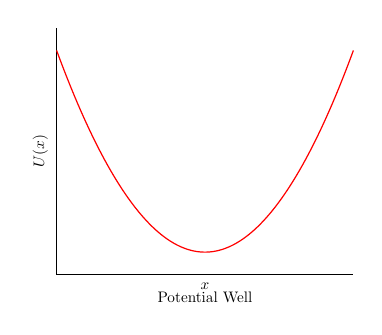
\begin{tikzpicture}[scale=0.55]
            \begin{axis}[
                axis lines=left,
                xlabel=$x$,
                ylabel=$U(x)$,
                ymin=-1, ymax=10,
                xtick=\empty, ytick=\empty,
                axis line style={-},
                clip=false
            ]
            \addplot [
                domain=-3:3,
                samples=100,
                color=red,
                thick,
            ]
            {x^2};
            \node at (axis cs:0, -2) {Potential Well};
            \end{axis}
        \end{tikzpicture}
        \end{minipage}
        \begin{minipage}{0.4\textwidth}    
        \begin{tikzpicture}[scale=0.55]
            \begin{axis}[
                axis lines=left,
                xlabel=$x$,
                ylabel=$P(x)$,
                ymin=0, ymax=1.25,
                xtick=\empty, ytick=\empty,
                axis line style={-},
                clip=false
            ]
            \addplot [
                domain=-3:3,
                samples=100,
                color=blue,
                thick,
            ]
            {exp(-x^2)};
            \node at (axis cs:0, -0.25) {Stationary PDF};
            \end{axis}
        \end{tikzpicture}
        \end{minipage}
    \end{center}
    \end{exampleblock}

\subsection{The Probability Current}
The Fokker-Planck equation can also be interpreted from a different, physically intuitive perspective. Recall its general form:

\vspace{-0.75em}

\small
$$
\partial_t P = \partial_x \left[ -a(x)P(x,t) - \partial_x \left( \frac{b(x)^2}{2}P(x,t) \right) \right]
$$
\normalsize
If we factor out the outer derivative and define the expression inside the brackets as $J$, we obtain:
$$
\partial_t P + \partial_x J = 0
$$
This is immediately recognizable as a continuity equation (or conservation law) for probability. In higher dimensions, the equation generalizes to:
$$
\partial_t \eta + \nabla \cdot J = 0
$$
where $\eta$ is the probability density and $J$ is the probability current (or flux vector).

This formulation highlights that the probability behaves like a conserved "fluid". The change in its distribution is nothing more than a redistribution, so the total amount does not change.

In one dimension, the continuity equation is a direct reduction of the multi-dimensional case. For example, in the case of pure Brownian motion (diffusion), the probability current takes the form:
$$
J = -K \nabla P
$$
where $K$ is the diffusion coefficient. Here, $J$ describes the net flow of probability due to diffusion, always moving from regions of high to low probability density. For this reason, $J$ is often referred to as the \textbf{probability current}.

\begin{exampleblock}[Particle density]

    We want to study how the spatial density $n(x,t)$ of a large number of particles evolves, where each particle follows the same stochastic dynamics:
    $$
    \begin{cases}
    \dot x_j = f(x_j) & \to \ \ drift\ term\\
    n(x,0) = \theta^*(x) & \to \ \ initial\ density
    \end{cases}
    $$
    We assume that particles are neither created nor destroyed, so the total number $N$ is conserved:
    $$
    \int_{\mathbb{R}} n(x,t)\, dx = N = \int_{\mathbb{R}} n(x,0)\, dx = \int_{\mathbb{R}} \theta^*(x)\, dx
    $$
    The motion takes place in $\mathbb{R}$. The probability that a particle is in $C = [a,b]$ at time $t$ is:
    $$
    \Pr [x(t) \in [a,b]] \simeq \frac{N_c(t)}{N} = \frac{\int_a^b n(x,t)\, dx}{N}
    = \frac{\# \text{ particles in } [a,b]}{\# \text{ particles in } \mathbb{R}}
    $$
    Thus, the probability density is:
    $$
    \rho(x,t) = \frac{n(x,t)}{N}
    $$

    \vspace{0.5em}

    \textbf{Evolution of $\mathbf{n(x,t)}$}

    \vspace{0.5em}

    Consider now an infinitesimal interval $[x, x+dx]$, and let $Q_x = N_{[x, x+dx]}$ be the number of particles in it.
    Since each particle evolves according to $\dot x = f(x)$, the velocity at position $x$ is:
    $$
    v(x) = f(x)
    $$
    The particle fluxes are:

    \begin{enumerate}
        \item Number of \bfit{particles entering} $[x, x+dx]$ per unit time:
        $\quad
        n(x,t)\, v(x)\, dt
        $
        \item Number of \bfit{particles leaving} $[x, x+dx]$ per unit time:
        $\quad \ 
        n(x+dx,t)\, v(x+dx)\, dt
        $
    \end{enumerate}

    \vspace{0.5em}

    The net change in particle number in $[x, x+dx]$ is:
    $$
    dQ = n(x,t)v(x)\,dt - n(x+dx,t)v(x+dx)\,dt
    $$
    Dividing by $dt$ and using a Taylor expansion of $n(x+dx,t)$ around $x$:
    $$
    \frac{dQ}{dt} = - \partial_x [n(x,t)v(x)]\, dx
    $$
    but $Q_{[x, x+dx]} = n(x,t)\,dx$, so:
    $$
    \frac{\partial}{\partial t} n(x,t)\, dx = - \partial_x [n(x,t)v(x)]\, dx
    $$
    Dividing both sides by $dx$ gives the following system:
    $$
    \begin{cases}
        \dfrac{\partial n}{\partial t} + \dfrac{\partial}{\partial x} [v(x)n(x,t)] = 0\\
        n(x,0) = \theta^*(x)\\
        \displaystyle\int n(x,t)\, dx = N
    \end{cases}
    $$

    This is the \bfit{Liouville equation} for the normalized density $\frac{n(x,t)}{N}$.

    \vspace{0.5em}

    \textbf{The probability current}

    \vspace{0.4em}

    We now introduce two key quantities:

    \vspace{0.4em}

    \begin{enumerate}[leftmargin=*]
        \item $n(x,t)\,dx$: \# of particles in the interval $(x, x + dx)$ at time $t$.
        \item $J(x,t) = n(x,t)\,v(x)$: \# of particles crossing position $x$ at time $t$, (\bfit{current density}).
    \end{enumerate}

    \vspace{0.4em}

    The net change in the number of particles in $[x, x+dx]$ over time $dt$ is:
    $$
    dQ = J(x,t)\,dt - J(x+dx,t)\,dt
    $$

    This leads to the continuity equation:
    $$
    \partial_t n = -\partial_x J \qquad \Rightarrow \qquad \partial_t n + \partial_x J = 0
    \qquad \xrightarrow{\text{in } \mathbb{R}^2} \qquad \partial_t n + \text{div}\, J = 0
    $$

    The FP equation can also be interpreted as describing the evolution of the spatial density of a large amount of particles, each subject to a white noise force and an initial density $\theta(x)$:
    $$
    \partial_t n(x,t) = -\partial_x\big(f(x)\,n(x,t)\big) + \partial_{xx}^2\left(\frac{g^2(x)}{2}\,n(x,t)\right)
    $$
    where $n$ is normalized so that $\int_{\mathbb{R}} n(x,t)\,dx = N = \int_{\mathbb{R}} \theta(x)\,dx$.

    If each particle evolves according to $\dot{x} = f(x) + g(x)\,\xi(t)$, the particle current is:
    $$
    J = f(x)\,n(x,t) - \partial_x\left(\frac{g^2(x)}{2}\,n(x,t)\right)
    $$

    The analogous expression for the \bfit{probability current} (using normalized density $\rho(x,t)$) is:
    $$
    J_{\text{prob}} = f(x)\,\rho(x,t) - \partial_x\left(\frac{g^2(x)}{2}\,\rho(x,t)\right)
    $$
    
\end{exampleblock}


\subsection{Special Cases of the Fokker-Planck Equation}

\subsubsection{Deterministic Systems with Random Initial Conditions}
Suppose we have a deterministic system, $\dot{x} = a(x)$, but where the initial conditions are described by a probability distribution $\theta(x)$. Here, randomness comes only from the initial condition, not from noise in the dynamics: the diffusion coefficient is zero, $b(x)=0$. The Fokker-Planck equation loses its second-order derivative term and becomes the \textbf{Liouville equation}:
\small
$$
\begin{cases}
    \dfrac{\partial P(x,t)}{\partial t} = -\dfrac{\partial}{\partial x}\left(a(x)P(x,t)\right) \\[0.8em]
    P(x,0) = \theta(x)
\end{cases}
$$
\normalsize
This type of problem appears, for example, when studying the evolution of a population's distribution over time under deterministic laws, but starting from a known initial distribution.

\subsubsection{Purely Diffusive Systems}
The opposite case occurs when $a(x)=0$, and the system is governed only by noise:
$$
dx = b(x)dW
$$
In population dynamics, this is useful in cases where the baseline growth rate is zero ($r=0$) or constant. In this situation, the Fokker-Planck equation becomes a pure diffusion equation:
$$
\partial_t P = \partial_x^2 \left( \frac{b(x)^2}{2} P(x,t) \right)
$$
This is, in fact, a generalization of the process for the Wiener process, which I recall is $\dot{w} = \xi(t)$ (i.e., $a=0, b=1$). Indeed, using the Fokker-Planck equation, we can find the expression for the PDF of the Wiener process, which will be:
$$
\partial_t P = \frac{1}{2} \partial_w^2 P
$$
Or, analogously, for $\dot{x} = \omega\xi(t)$, which corresponds to the overdamped Brownian motion:
$$
\partial_t P = \frac{\omega^2}{2} \partial_x^2 P
$$

\subsubsection{Kac's Lemma} \label{sec:kac}

Kac's Lemma establishes a fundamental relationship between stationary probabilities and expected return times in ergodic stochastic processes. Consider a stationary Markov process with stationary distribution $\pi$ and let $A$ be a measurable subset of the state space. Define $T_A$ as the first return time to $A$ when starting from a point in $A$. Kac's Lemma states:

$$
\mathbb{E}[T_A | X_0 \in A] = \frac{1}{\pi(A)}
$$

where $\pi(A) = \int_A \pi(x) dx$ is the stationary measure of set $A$.

This result provides a direct connection between the equilibrium properties of the system (captured by $\pi$) and its dynamical properties (captured by return times). States or regions with low stationary probability have correspondingly long expected return times.

The lemma follows from the ergodic theorem: for an ergodic process, the long-run proportion of time spent in any set equals its stationary probability. Since visits to $A$ occur approximately every $\mathbb{E}[T_A]$ time units, we have $\pi(A) \approx 1/\mathbb{E}[T_A]$.

\subsection{Multiple Independent Noises}

Consider the following Itô stochastic differential equation (SDE) with two independent noise sources:
$$
dx = a(x)\,dt + b_1(x)\,dW_1 + b_2(x)\,dW_2
$$
where $dW_1$ and $dW_2$ are independent Wiener processes (i.e., uncorrelated Brownian motions).

The associated Fokker-Planck equation (FPE) for the probability density $P(x,t)$ is obtained by extending the standard procedure for a single noise term. The result is:
$$
\partial_t P(x, t) = -\partial_x \left( a(x) P(x, t) \right)
+ \partial_{xx}^2 \left( \frac{b_1^2(x) + b_2^2(x)}{2} P(x, t) \right)
$$
In other words, the diffusion coefficients from each independent noise source add together in the FPE. This generalizes immediately to any number of independent noises: the total diffusion is the sum of the squared amplitudes of each noise term.

\begin{exampleblock}[RL Circuit with Multiple Noise Sources]
Consider an RL circuit where both the external magnetic field and the resistance fluctuate independently. We start with a circuit perturbed by fluctuating external magnetic fields $\Phi_{ext}$ such that $(d/dt)\Phi_{ext}$ is white noise:
$$
\frac{dI}{dt} = -\frac{R}{L}I + \omega_1\xi_1(t)
$$

However, the resistance is not constant; it fluctuates due to thermal agitation, which we model as white noise:
$$
R \to R + K\xi_2(t)
$$

This yields the following model:
$$
\frac{dI}{dt} = -\frac{R + K\xi_2(t)}{L}I + \omega_1\xi_1(t)
$$

Expanding this expression:
$$
\frac{dI}{dt} = -\frac{R}{L}I - \frac{K}{L}I\xi_2(t) + \omega_1\xi_1(t)
$$

In this model, the noise is not only additive but also multiplicative. We have two independent noise sources: $\xi_1(t)$ (additive) from the magnetic field fluctuations and $\xi_2(t)$ (multiplicative) from the resistance fluctuations. The total noise contribution combines both effects according to the rules we have established for multiple independent noises.
\end{exampleblock}

\newpage

\section{Multiplicative Noise}

While additive noise provides a good model for systems perturbed by external forces, many real-world systems feature fluctuations whose intensity depends on the state of the system itself. This leads to the concept of \textbf{multiplicative noise}, which can induce much richer and more complex behaviors than its additive counterpart.

Consider a system governed by a parameter $p$. The simplest case is when it is possible to write the field in the form
$$
\dot{x} = b(x) + p \hat{g}(x)
$$
that is, with linear dependence on the parameter considered. The parameter $p$ is usually influenced by the external world, so in some cases it is possible for it to become stochastic. We can then describe a stochastic $p$ as
$$
p \to p + \alpha \xi(t)
$$
Substituting, we obtain
$$
\dot{x} = b(x) + p \hat{g}(x) + \hat{g}(x) \alpha \xi(t)
$$
We can then group the stochastic terms, obtaining
$$
\dot{x} = f(x) + g(x) \xi(t)
$$
The \textbf{Fokker-Planck equation} for the general case is:
$$
\frac{\partial \rho}{\partial t} = - \frac{\partial}{\partial x} [f(x) \rho] + \frac{\partial^2}{\partial x^2} \left[ \frac{g(x)^2}{2} \rho \right]
$$
So far, we have only considered cases where $g(x)$ is constant. Here, however, we are dealing with the most general version of what we have seen so far. The boundary conditions remain the same as before, and as usual, we analyze the stationary case. We have:
$$
\frac{d}{dx} \left[ \frac{g(x)^2}{2} P_s(x) \right] = f(x)P_s(x)
$$
This is a first-order ODE that can be solved for $P_s(x)$. 

Let's define an auxiliary function $Q(x) = \frac{g(x)^2}{2} P_s(x)$. The equation becomes:
$$
\frac{dQ}{dx} = f(x) \frac{2}{g(x)^2} Q(x)
$$
This is a standard linear ODE of the form $Q'(x) = a(x)Q(x)$, whose solution is $Q(x) = C e^{A(x)}$, where $A(x) = \int a(s)ds$. Applying this, we find:
$$
Q(x) = C \exp\left( \int \frac{2f(s)}{g(s)^2} ds \right)
$$
Substituting back $P_s(x) = \frac{2}{g(x)^2}Q(x)$, we arrive at the general solution for the stationary PDF:
$$
P_s(x) = \frac{C'}{g(x)^2} \exp\left( \int^x \frac{2f(z)}{g(z)^2} dz \right)
$$
where $C'$ is a normalization constant. Let's remark that, being a probability density, the integral of $P_s(x)$ over the entire state space must be equal to one.

We can distinguish two cases:
\begin{itemize}
    \item If the integral exists (is finite), then everything is fine and we can calculate $C$ to normalize $P_s(x)$.
    \item If instead the integral is infinite, we can only find a formal solution that has no physical meaning: in this case it is necessary to study the steady state directly starting from the SDE (\cref{sec:nit}). 
\end{itemize}

\section{Multiplicative Noise: Noise-Induced Transitions} \label{sec:nit}

In the case of additive noise ($g(x) = \text{const}$), the extrema of the stationary PDF $P_s(x)$ coincide with the equilibria of the deterministic system (where $f(x)=0$). With multiplicative noise, this simple correspondence breaks down. Recalling the following identity:
$$
\dfrac 1{g^2(x)} = e^{-\ln g^2(x)} = e^{-2 \ln g(x)}
$$
We can rewrite the stationary probability density function in a more transparent exponentialform:
$$
P_s(x) = 2 C \exp \left\{
    - 2 \log (g(x)) + \int_\alpha^x \dfrac{2 f(s)}{g^2(s)} ds
\right\}
$$
This highlights how both the noise amplitude $g(x)$ and the drift $f(x)$ contribute to shaping the stationary distribution. To investigate the location of the extrema of $P_s(x)$, we differentiate with respect to $x$. Applying the chain rule to the exponent, we obtain:
$$
P_s'(x) = 2 C \exp \left\{
    - 2 \dfrac{g'(x)}{g(x)} + \dfrac{2 f(x)}{g^2(x)}
    \right\}
$$
This expression will allow us to determine where the stationary distribution attains its maxima and minima, as these correspond to the points where $P_s'(x) = 0$.

To find the extrema of $P_s(x)$, we must find where its derivative is zero, $P_s'(x)=0$. After some algebraic manipulation of the general solution, this condition simplifies to:
$$
f(x) \ge g(x)g'(x)
$$
Of course, if $g(x)$ is constant, then $g'(x) = 0$ and the condition reduces to $f(x) \geq 0$. This immediately recovers the familiar property that stable equilibria correspond to modes of the PDF, and unstable equilibria correspond to antimodes.

Instead, the most interesting case is when $g(x)$ is not constant. In this case, the condition $f(x) \ge g(x)g'(x)$ is a non-linear inequality that can have multiple solutions. This means that by simply varying a parameter that controls the noise intensity, new extrema can appear in the PDF that were completely absent in the unperturbed deterministic system. This phenomenon, discovered by Horsthemke and Lefever in the 1970s, is called a \textbf{Noise-Induced Transition (NIT)}.

Before the discovery of NITs, it was commonly believed that noise could only act in two ways:
\begin{itemize}
    \item In unimodal systems, it creates a "cloud" of fluctuations around a single deterministic equilibrium.
    \item In multimodal systems, it can cause "jumps" between the existing deterministic equilibria.
\end{itemize}
NITs showed that noise can play a much more constructive role, inducing oscillations and creating entirely new states that are not present in the unperturbed deterministic system.

\begin{observationblock}[Extrema vs. Equilibria]
    Even if solving
    $$f(x) = g'(x,q)g(x,q)$$
    one does find as extrema for the stochastic model as the equilibria for the deterministic system, the extrema of the stationary PDF do not correspond to equilibrium points of the deterministic equation, which solved a different equilibrium equation, namely:
    $$f(x) = 0$$
    \end{observationblock}

\begin{exampleblock}[Noise-Induced Bifurcation in Gene Expression]
Consider a simple model for protein production, where a protein X acts as its own transcription factor. The production rate is $Q(x)$ and the degradation rate is $dx$.
$$
\dot{x} = Q(x) - dx
$$
A common form for $Q(x)$ that models self-regulation is:
$$
Q(x) = R + K\frac{x^2}{K_d + x^2}
$$
where $R$ is a basal production rate and the second term is a Hill function describing feedback. The deterministic system is:
$$
\dot{x} = \underbrace{R + K\frac{x^2}{K_d + x^2} - dx}_{f(x)}
$$
For small degradation rates $d$, this system has a single, globally stable equilibrium point.

Now, suppose the degradation rate $d$ is subject to stochastic fluctuations: $d \to d + \alpha\xi(t)$. The SDE becomes:
$$
dx = \left(R + K\frac{x^2}{K_d + x^2} - dx\right)dt - \alpha x dW_t
$$
Here, the noise is multiplicative, with $g(x) = -\alpha x$, so $g'(x) = -\alpha$. The condition for the extrema of the stationary PDF, $f(x) \ge g(x)g'(x)$, is:
$$
R + K\frac{x^2}{K_d + x^2} - dx \ge (-\alpha x)(-\alpha) = \alpha^2 x
$$
Rearranging gives:
$$
R + K\frac{x^2}{K_d + x^2} \ge (d + \alpha^2)x
$$
Depending on the value of the noise parameter $\alpha$, this algebraic equation can have one or three solutions. This means that by changing the noise intensity, the stationary PDF can transition from being unimodal (with one peak) to bimodal (with two peaks), even though the underlying deterministic system only had one equilibrium point. This is a classic example of a noise-induced transition: the noise itself creates new, stable macroscopic states for the system.

\begin{figure}[H]
    \centering
    \includegraphics[width=0.45\textwidth]{assets/nit-1.png}
    \includegraphics[width=0.45\textwidth]{assets/nit-2.png}
    \caption{Left: Unimodal stationary PDF for null noise intensity $\alpha = 0$. Right: Bimodal stationary PDF emerging for higher noise intensity $\alpha$, demonstrating a noise-induced transition where new stable states appear that are absent in the deterministic system.}
\end{figure}

\end{exampleblock}

\newpage

\subsection{Perturbation of the Logistic Growth Model}
Let's revisit the logistic growth model, which serves as another prime example of how multiplicative noise can fundamentally alter a system's behavior. We start with the deterministic logistic equation:
$$
\dot{z} = r_1 z - r_2 z^2
$$
Through a linear change of variables $x = r_2 z$, we can adimensionalize the equation to a simpler form:
$$
\dot{x} = r x - x^2
$$
Now, we introduce stochasticity by perturbing the intrinsic growth rate, $r \to r + \omega\xi(t)$. This leads to the corresponding Itô equation with multiplicative noise:
$$
dx = (r x - x^2)dt + \omega x dW_t
$$
This defines our drift and diffusion coefficients as $f(x) = r x - x^2$ and $g(x) = \omega x$.

The stationary Fokker-Planck equation for this system is:
$$
\frac{d}{dx} \left[ \frac{g(x)^2}{2} P_s(x) \right] = f(x)P_s(x)
$$
Substituting our specific $f(x)$ and $g(x)$ gives:
$$
\frac{d}{dx} \left[ \frac{\omega^2 x^2}{2} P_s(x) \right] = (r x - x^2)P_s(x)
$$

To solve this differential equation, we can use the substitution method. Let $Q = x^2 P_s$, then:
$$
Q' = \frac{2r-x}{\omega^2 x} Q
$$
This can be rewritten as:
$$
\frac{dQ}{Q} = \frac{2r-x}{\omega^2 x} dx = \left[\frac{2r}{\omega^2 x} - \frac{1}{\omega^2}\right] dx
$$
Integrating both sides:
$$
\ln Q = \frac{2r}{\omega^2} \ln x - \frac{x}{\omega^2} + C
$$
Taking the exponential:
$$
Q(x) = A \exp\left[\frac{2r}{\omega^2} \ln x - \frac{x}{\omega^2}\right] = A x^{\frac{2r}{\omega^2}} e^{-\frac{x}{\omega^2}}
$$
Since $Q = x^2 P_s$, we obtain:
$$
P_s(x) = \frac{Q(x)}{x^2} = A x^{\frac{2r}{\omega^2}-2} e^{-\frac{x}{\omega^2}}
$$
where $A$ is a normalization constant.


A crucial step is to check whether this candidate solution is a valid, normalizable probability distribution. The integral $\int_0^\infty P_s(x) dx$ must be finite.
$$
\int_0^\infty x^{\frac{2r}{\omega^2}-2} e^{-\frac{2}{\omega^2}x} dx
$$
This is a form of the Gamma function integral, $\int_0^\infty t^{k-1}e^{-t}dt$. For this integral to converge at the lower bound ($x \to 0$), the exponent of $x$ must be greater than -1.
$$
\frac{2r}{\omega^2}-2 > -1 \quad \implies \quad \frac{2r}{\omega^2} > 1 \quad \implies \quad r > \frac{\omega^2}{2}
$$

This is valid only if $r > \omega^2/2$ as we have already seen in the past. If this does not hold, we cannot integrate but what does this actually mean? To understand this, let's return to the SDE:
$$
dx = x(r - x)dt + \omega x dW
$$

Applying now the transformation $y = \psi(x) = \log x$, then $\psi'(x) = x^{-1}$ and $\psi''(x) = -x^{-2}$. Therefore:
$$
dy = \left[\frac{1}{\cancel{x}}x(r - x) - \frac{1}{\cancel{x^2}} \frac{\omega^2 \cancel{x^2}}{2}\right]dt + \omega dW
$$

Therefore, substituting in $y$:
$$
dy = \left[r - \frac{\omega^2}{2} - e^y\right]dt + \omega dW
$$

Integrating then:
$$
y(t) = y_0 + \left(r - \frac{\omega^2}{2}\right)t - \int_0^t e^{y(s)}ds + \omega[W(t) - W(0)]
$$

Notice that the integral term, $-\int_0^t e^{y(s)}ds$, is always negative (since $e^{y(s)} > 0$ for all $s$). 

\begin{itemize}

    \item \textbf{Case 1:} $r < \omega^2/2$

    If $r < \omega^2/2$, the drift term $\left(r - \frac{\omega^2}{2}\right)t$ is negative and dominates for large $t$, while the stochastic term becomes negligible in comparison. As a result, $y(t) \to -\infty$ as $t \to \infty$, which means $x(t) = e^{y(t)} \to 0^+$. In this regime, the probability distribution $P(x, t)$ collapses to a delta function at zero:
$$
    \lim_{t \to \infty} P(x, t) = \delta(x)
$$
This shows that, in this case, the Fokker-Planck equation predicts a stationary solution, but in reality, all probability accumulates at extinction ($x=0$). Thus, the Fokker-Planck approach alone can be misleading for this parameter regime.

    \item \textbf{Case 2:} $r > \omega^2/2$

    On the other hand, when $r > \omega^2/2$, the stationary solution is normalizable and given by:
    $$
        P_s(x) = A x^{\frac{2r}{\omega^2}-2} e^{-\frac{2}{\omega^2}x}
    $$

\end{itemize}


\begin{figure}[H]
    \centering
    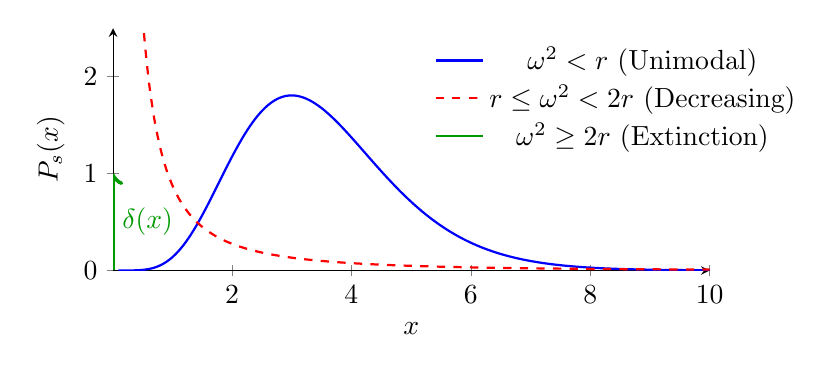
\begin{tikzpicture}
        \begin{axis}[
            scale=0.9,
            width=10cm,
            height=5cm,
            axis lines=left,
            xlabel={$x$},
            ylabel={$P_s(x)$},
            xmin=0.01, xmax=10,
            ymin=0, ymax=2.5,
            legend pos=north east,
            legend style={draw=none, fill=none, xshift=1.5cm},
        ]
        % Case 1: Unimodal PDF (r1 > omega^2)
        \addplot[domain=0.1:10, samples=100, color=blue, thick, smooth] {x^(2*4/1-2)*exp(-2/1*x)};
        \addlegendentry{$\omega^2 < r$ (Unimodal)};
        
        % Case 2: Decreasing PDF (r1 <= omega^2 < 2r1)
        \addplot[domain=0.1:10, samples=100, color=red, thick, smooth, dashed] {x^(2*4/16-2)*exp(-2/16*x)};
        \addlegendentry{$r \le \omega^2 < 2r$ (Decreasing)};
        
        % Case 3: Extinction (delta function, illustrative) - invisible plot for legend
        \addplot[draw=none, color=green!60!black] coordinates {(0,0)};
        \addlegendentry{$\omega^2 \ge 2r$ (Extinction)};
        
        % Case 3: Extinction (delta function, illustrative) - visual representation
        \draw[->, ultra thick, green!60!black] (0.01,0) -- (0.01,1);
        \node[green!60!black, right] at (0, 0.5) {$\delta(x)$};
        
        \end{axis}
    \end{tikzpicture}
    \caption{Noise-Induced Transition in the logistic model.}
\end{figure}


Let us also consider two special cases:
\begin{itemize}
    \item If $\omega^2 = 2r$ (i.e., $2r/\omega^2 = 1$), the stationary distribution simplifies to:
    $$
        P_s(x) = A x^{-1} e^{-\frac{x}{r}}
    $$
    \item If there is no noise, $\omega^2 = 0$, the stationary distribution becomes:
    $$
        P_s(x) = A e^{-\frac{x}{r}}
    $$
    This change has a significant effect on the shape of the stationary distribution. Specifically, when the parameters satisfy
    $$
        \frac{2r}{\omega^2} < 2 \qquad \text{or equivalently} \qquad r < \frac{\omega^2}{2}
    $$
    the distribution $P_s(x)$ is no longer unimodal (with a peak at some $x > 0$), but instead becomes a monotonically decreasing function of $x$. In this regime, the probability density is highest near $x=0$ and decreases for larger $x$, so the system is most likely to be found close to $x=0$.
\end{itemize}


Furthermore, it can be shown that the stationary distribution $P_s(x)$ is normalizable (i.e., its total probability integrates to 1) only if $\omega^2 < 2r$. This is consistent with the more general result discussed in the previous section.

\section{The Stratonovich Integral}

The Langevin equation, $\dot{x} = a(x,t) +b(x,t) \xi(t)$, provides an intuitive starting point, but its rigorous interpretation requires us to define the stochastic integral $\int b(x,t)dW_t$. This is best understood by rewriting the SDE in its formal integral form:
$$
x(t) = x(0) + \int_0^t a(x(\theta),\theta) d\theta + \int_0^t b(x(\theta),\theta) dW(\theta)
$$
As we will see, the very definition of the final term, the stochastic integral, is ambiguous and has led to two major, distinct formulations of stochastic calculus: Itô and Stratonovich.

\subsection{The Ambiguity of the Stochastic Integral}

The integral of a function with respect to a Wiener process, $I = \int_0^t g(X(\theta)) dW(\theta)$, cannot be defined in the ordinary Riemann sense because the path of $W(t)$ is nowhere differentiable and not of bounded variation. Instead, it is defined as the limit of a Riemann-Stieltjes sum over a partition of the interval $[0, t]$. Let us partition $[0, t]$ into $N$ subintervals with points $0 = t_0 < t_1 < \ldots < t_N = t$, and let $J = \max_{i} (t_i - t_{i-1})$ denote the maximum interval length of the partition. For each subinterval, we choose an evaluation point $\tau_i \in [t_{i-1}, t_i]$. The stochastic integral is then defined as the limit (in probability) as $J \to 0$ of the sum:
$$
S(J) = \sum_{i=1}^N g(X(\tau_i)) \left[ W(t_i) - W(t_{i-1}) \right]
$$
where $S(J)$ is a random variable for each partition.

If $W(t)$ were a deterministic, smooth function, the choice of $\tau_i$ would not matter in the limit $J \to 0$. However, because $W(t)$ is a random process with highly irregular paths, the value of the stochastic integral depends crucially on the choice of $\tau_i$.

To illustrate this, consider the specific case $I = \int_0^t W(\theta) dW(\theta)$. The corresponding sum is:
$$
S(J) = \sum_{i=1}^N W(\tau_i) \left[ W(t_i) - W(t_{i-1}) \right]
$$
Let us compute the expected value of this sum:
$$
\langle S(J) \rangle = \sum_{i=1}^N \langle W(\tau_i) \left[ W(t_i) - W(t_{i-1}) \right] \rangle = \sum_{i=1}^N \left( \langle W(\tau_i) W(t_i) \rangle - \langle W(\tau_i) W(t_{i-1}) \rangle \right)
$$
Using the autocorrelation property of the Wiener process, $\langle W(t) W(s) \rangle = \min(t, s)$, and noting that $t_{i-1} \leq \tau_i \leq t_i$, we have:
$$
\langle S(J) \rangle = \sum_{i=1}^N \left( \min(\tau_i, t_i) - \min(\tau_i, t_{i-1}) \right) = \sum_{i=1}^N (\tau_i - t_{i-1})
$$
Thus, the expected value depends on the choice of $\tau_i$ within each interval. If we parameterize $\tau_i$ as
$$
\tau_i = t_{i-1} + \alpha (t_i - t_{i-1}), \qquad \alpha \in [0, 1],
$$
and consider a uniform partition where $J = t_i - t_{i-1} = t/N$, then
$$
\tau_i - t_{i-1} = \alpha J,
$$

so

$$
\langle S(J) \rangle = \sum_{i=1}^N \alpha J = \alpha N \frac tN = \alpha t.
$$
Taking the limit as $J \to 0$ (i.e., $N \to \infty$ and $J \to 0$), we see that
$$
\langle I \rangle = \lim_{J \to 0} \langle S(J) \rangle = \alpha t.
$$
Therefore, the expectation of the stochastic integral depends directly on the convention used for the evaluation point $\alpha$. This ambiguity in the definition of the stochastic integral is fundamental and necessitates a choice of interpretation.

\begin{itemize}
    \item The \textbf{Itô Integral} convention chooses $\alpha=0$, evaluating the integrand at the start of the interval ($\tau_i = t_{i-1}$). This ensures the integrand is independent of the future noise increment, making the resulting stochastic integral a martingale.
    \item The \textbf{Stratonovich Integral} convention chooses $\alpha=1/2$, evaluating the integrand at the midpoint of the interval ($\tau_i = (t_{i-1}+t_i)/2$). This choice makes the rules of calculus for the integral resemble ordinary calculus.
\end{itemize}

\newpage

\subsection{Choosing a Convention: The Wong-Zakai Theorem}
The choice between Itô and Stratonovich is not merely a mathematical preference; it is a modeling decision. The \textbf{Wong-Zakai theorem} provides crucial guidance.

\begin{definitionblock}[Wong-Zakai Theorem (1965)]
    Consider an ODE perturbed by "real" noise $\eta_\epsilon(t)$ that is not perfectly white but has a very short correlation time $\epsilon$:
    $$ \dot{x} = a(x) + b(x)\eta_\epsilon(t) $$
    As the correlation time of the noise approaches zero ($\epsilon \to 0$), so that $\eta_\epsilon(t)$ converges to a true white noise process, the solution $x(t)$ of the ODE converges to the solution of the \textbf{Stratonovich SDE}, denoted by:

    $$ dx = a(x)dt + b(x) \circ dW_t $$
\end{definitionblock}

\begin{tipsblock}[When to use which integral?]
The Wong-Zakai theorem implies that if an SDE is derived as the limit of a physical system driven by noise with a finite (even if very small) correlation time, the Stratonovich interpretation is the more physically appropriate one. The Itô calculus is often preferred in mathematical finance and for problems where the noise is assumed to be idealized white noise from the outset, or for systems with intrinsically discrete state variables (like population counts).
\end{tipsblock}

\subsection{Connecting the Itô and Stratonovich SDEs}
We can find a direct relationship between the two formalisms by expanding the midpoint term in the Stratonovich definition.
First, we approximate the state at the midpoint:
$$
x\left(t+\frac{dt}{2}\right) \approx x(t) + a(x(t))\frac{dt}{2} + b(x(t))\left(W\left(t+\frac{dt}{2}\right) - W(t)\right)
$$
Next, we expand the function $b$ around $x(t)$:
$$
b\left(x\left(t+\frac{dt}{2}\right)\right) \approx b(x(t)) + b'(x(t)) \left( x\left(t+\frac{dt}{2}\right) - x(t) \right)
$$
Substituting the first expression into the second gives:
$$
b\left(x\left(t+\frac{dt}{2}\right)\right) \approx b(x(t)) + b'(x(t))\left[ a(x(t))\frac{dt}{2} + b(x(t))\hat{dW} \right]
$$
where $\hat{dW} = W(t+\frac{dt}{2}) - W(t)$. Now we substitute this back into the Stratonovich SDE definition:
$$
dx = a(x)dt + \left( b(x) + b'(x)\left[ a(x)\frac{dt}{2} + b(x)\hat{dW} \right] \right) dW_t
$$
Expanding this, we get three terms involving $dW_t$:
$$
dx = a(x)dt + b(x)dW_t + a(x)b'(x)\frac{dt}{2}dW_t + b(x)b'(x)\hat{dW}dW_t
$$
The term $dt\,dW_t$ is of order $O(dt^{3/2})$ and can be neglected. The final term requires us to evaluate the expectation $\langle\hat{dW}dW_t\rangle$.
$$
\langle \hat{dW}dW_t \rangle = \left\langle \left(W(t+\frac{dt}{2}) - W(t)\right)\left(W(t+dt) - W(t)\right) \right\rangle = \min\left(t+\frac{dt}{2}, t+dt\right) - t = \frac{dt}{2}
$$
where the minimum comes from the autocorrelation of the Wiener process $\langle W(t)W(s) \rangle = \min(t, s)$.

\vspace{0.5em}

Therefore, the term $b(x)b'(x)\hat{dW}dW_t$ contributes a drift of $\frac{1}{2}b(x)b'(x)dt$.
Combining all terms, the Stratonovich SDE is equivalent to the following Itô SDE:
$$
dx = \left( a(x) + \frac{1}{2}b(x)b'(x) \right)dt + b(x)dW_t
$$

\begin{definitionblock}[Stratonovich-to-Itô Conversion]
A Stratonovich SDE
$$
dx = a(x)dt + b(x)\circ dW_t
$$
is equivalent to an Itô SDE with a modified drift term:
$$
dx = \left( a(x) + \frac{1}{2}b(x)b'(x) \right)dt + b(x)dW_t
$$
This conversion formula allows us to switch between the two calculi, leveraging the strengths of each. The extra drift term $\frac{1}{2}b(x)b'(x)$ is often called the "noise-induced drift" or "spurious drift."
\end{definitionblock}

\subsection{Fokker-Planck Equation for Stratonovich SDEs}

Given the conversion formula, we can easily find the Fokker-Planck equation for a Stratonovich SDE. We simply take the Fokker-Planck equation for an Itô SDE and replace the drift $a(x)$ with the effective drift $a(x) + \frac{1}{2}b(x)b'(x)$.

$$
\frac{\partial \rho}{\partial t} = - \frac{\partial}{\partial x} \left[ \left(a(x) + \frac{1}{2}b(x)b'(x)\right)\rho \right] + \frac{1}{2} \frac{\partial^2}{\partial x^2} \left[ b(x)^2 \rho \right]
$$

This equation can be rewritten in a more compact and elegant form. Noting that $b(x)b'(x) = \frac{1}{2}\frac{d}{dx}(b(x)^2)$, we can combine the terms:

$$
\frac{\partial \rho}{\partial t} = - \frac{\partial}{\partial x} [a(x)\rho] + \frac{1}{2} \left( -\frac{\partial}{\partial x}\left[\frac{d(b^2)}{dx}\rho\right] + \frac{\partial^2}{\partial x^2}[b^2\rho] \right)
$$

Let us use the product rule on the second derivative:

$$
\frac{\partial^2}{\partial x^2} [b^2 \rho] = \frac{\partial}{\partial x} \left( \frac{\partial (b^2)}{\partial x} \rho + b^2 \frac{\partial \rho}{\partial x} \right) = \frac{\partial^2 (b^2)}{\partial x^2} \rho + 2 \frac{\partial (b^2)}{\partial x} \frac{\partial \rho}{\partial x} + b^2 \frac{\partial^2 \rho}{\partial x^2}
$$
Now, consider the term

$$
- \frac{\partial}{\partial x} \left[ \frac{\partial (b^2)}{\partial x} \rho \right] + \frac{\partial^2}{\partial x^2} [b^2 \rho]
$$

Substituting the expanded form, we get:
$$
\frac{\partial \rho}{\partial t} = - \left( \frac{\partial^2 (b^2)}{\partial x^2} \rho + \frac{\partial (b^2)}{\partial x} \frac{\partial \rho}{\partial x} \right) + \left( \frac{\partial^2 (b^2)}{\partial x^2} \rho + 2 \frac{\partial (b^2)}{\partial x} \frac{\partial \rho}{\partial x} + b^2 \frac{\partial^2 \rho}{\partial x^2} \right)
$$

Canceling the common terms, we are left with:

$$
\frac{\partial \rho}{\partial t} = \frac{\partial (b^2)}{\partial x} \frac{\partial \rho}{\partial x} + b^2 \frac{\partial^2 \rho}{\partial x^2} = \frac{\partial}{\partial x} \left[ b \frac{\partial}{\partial x} (b \rho) \right]
$$

Therefore, the equation becomes:

$$
\frac{\partial \rho}{\partial t} = - \frac{\partial}{\partial x} [a(x)\rho] + \frac{1}{2} \frac{\partial}{\partial x} \left[ b(x) \frac{\partial}{\partial x} (b(x)\rho) \right]
$$

This is the common form of the Fokker-Planck equation found in many physics textbooks. It highlights that in the Stratonovich interpretation, the diffusion term has a simpler structure.

\subsubsection{The Stationary Distribution for Stratonovich SDEs}

The Stratonovich form turns out to be quite convenient when dealing with the stationary distribution $P_s$, since

$$
0 = -\frac{d}{dx}\left[a(x)P_s\right] + \frac{1}{2} \frac{d}{dx} \left[ b(x) \frac{d}{dx} (b(x)P_s) \right]
$$

By simplifying and rearranging, we easily obtain

$$
\frac{b(x)}{2} \frac{d}{dx} [b(x)P_s] = a(x)P_s
$$

Now, define $\mathcal{H} = b(x)P_s$ so that

$$
\frac{d\mathcal{H}}{dx} = \frac{2a(x)}{b(x)^2} \mathcal{H}
\implies
\mathcal{H} = C \exp\left[ \int_{x} \frac{2a(z)}{b(z)^2} dz \right]
$$

Therefore,

$$
P_s(x) = \frac{C}{b(x)} \exp\left[ \int_{x} \frac{2a(z)}{b(z)^2} dz \right]
= C \exp\left[ -\log(b(x)) + \int_{x} \frac{2a(z)}{b(z)^2} dz \right]
$$

Once again, we want a formula that allows us to calculate the stationary points, so we can verify that it is sufficient to consider the stationary points of the exponent:

$$
\frac{2a(x)}{b(x)^2} - \frac{b'(x)}{b(x)} \ge 0
\implies
a(x) \ge \frac{1}{2} b(x) b'(x)
$$

The only difference compared to the Itô formulation is the factor $1/2$. The difference is therefore only quantitative, not qualitative. We have seen that the transitions due to noise can emerge in a new way that depends on the parameterization, even if the positions of the maxima and minima and their values change by different factors.


\subsubsection{Applications of SSDEs}

Let us revisit the Malthusian growth model, which is described by
$$
\dot{x} = r x
$$
where $r$ is the growth rate.

Suppose now that the growth rate is subject to random fluctuations, so that $r \to r + \alpha \xi(t)$, where $\xi(t)$ is white noise. 

Now, let us assume that the noise is such that it is described in the Stratonovich sense. The equation becomes
$$
dx = r x dt + \alpha x \circ dW
$$
where $\circ$ denotes the Stratonovich integral. The corresponding Ito version of this formula is
$$
dx = \left(r x + \frac{\alpha^2}{2} x\right) dt + \alpha x dW
$$

If we now apply the logarithmic transformation $y = \ln x$, we obtain
$$
dy = \left(r + \cancel{\frac{\alpha^2}{2}} - \cancel{\frac{\alpha^2}{2}}\right) dt + \alpha dW = r dt + \alpha dW
$$

However, if we instead use the Ito interpretation from the start, the equation for $x$ is
$$
dx = r x dt + \alpha x dW
$$
which, under the transformation $y = \ln x$, gives
$$
dy = \left(r - \frac{\alpha^2}{2}\right) dt + \alpha dW
$$

This leads to a crucial difference between the two interpretations. 

\begin{itemize}
    \item \textbf{Itô case:} If $\frac{\alpha^2}{2} > r$, then the drift term in the equation for $y = \ln x$ becomes negative, so $y(t) \to -\infty$ as $t \to \infty$. This means $x(t) \to 0$, and the population will eventually go extinct even if $r > 0$.
    \item \textbf{Stratonovich case:} The noise-induced drift term cancels out, so extinction only occurs if $r < 0$. In other words, the population persists as long as the deterministic growth rate $r$ is positive, regardless of the noise strength.
\end{itemize}

This difference is significant: in the Itô interpretation, strong enough noise can drive the population extinct even when the average growth rate is positive, while in the Stratonovich interpretation, only a negative growth rate leads to extinction.

Which interpretation should be used? The answer depends on the nature of the noise and the modeling context. The Itô calculus is appropriate when the noise is idealized as perfectly white and uncorrelated in time. The Stratonovich calculus is more suitable when the noise has a finite correlation time or comes from a smooth, physical process. In real-world applications, the correct choice depends on the details of the system being modeled.

In summary, the choice between Itô and Stratonovich calculus is not just a technicality: it can fundamentally change the predicted behavior of stochastic models, especially for questions like extinction thresholds and long-term outcomes.